%===============================================================================
% LaTeX sjabloon voor de bachelorproef toegepaste informatica aan HOGENT
% Meer info op https://github.com/HoGentTIN/latex-hogent-report
%===============================================================================

\documentclass[dutch,dit,thesis]{hogentreport}

% TODO:
% - If necessary, replace the option `dit`' with your own department!
%   Valid entries are dbo, dbt, dgz, dit, dlo, dog, dsa, soa
% - If you write your thesis in English (remark: only possible after getting
%   explicit approval!), remove the option "dutch," or replace with "english".

\usepackage{lipsum} % For blind text, can be removed after adding actual content
\usepackage{listings}
\usepackage{xcolor}

\definecolor{codegreen}{rgb}{0,0.6,0}
\definecolor{codegray}{rgb}{0.5,0.5,0.5}
\definecolor{codepurple}{rgb}{0.58,0,0.82}
\definecolor{backcolour}{rgb}{0.95,0.95,0.92}

\lstdefinestyle{mystyle}{
    backgroundcolor=\color{backcolour},   
    commentstyle=\color{codegreen},
    keywordstyle=\color{magenta},
    numberstyle=\tiny\color{codegray},
    stringstyle=\color{codepurple},
    basicstyle=\ttfamily\footnotesize,
    breakatwhitespace=false,         
    breaklines=true,                 
    captionpos=b,                    
    keepspaces=true,                 
    numbers=left,                    
    numbersep=5pt,                  
    showspaces=false,                
    showstringspaces=false,
    showtabs=false,                  
    tabsize=2
}

\lstset{style=mystyle}

%% Pictures to include in the text can be put in the graphics/ folder
\graphicspath{{graphics/}}

%% For source code highlighting, requires pygments to be installed
%% Compile with the -shell-escape flag!
\usepackage[section]{minted}
%% If you compile with the make_thesis.{bat,sh} script, use the following
%% import instead:
%% \usepackage[section,outputdir=../output]{minted}
\usemintedstyle{solarized-light}
\definecolor{bg}{RGB}{253,246,227} %% Set the background color of the codeframe

%% Change this line to edit the line numbering style:
\renewcommand{\theFancyVerbLine}{\ttfamily\scriptsize\arabic{FancyVerbLine}}

%% Macro definition to load external java source files with \javacode{filename}:
\newmintedfile[javacode]{java}{
    bgcolor=bg,
    fontfamily=tt,
    linenos=true,
    numberblanklines=true,
    numbersep=5pt,
    gobble=0,
    framesep=2mm,
    funcnamehighlighting=true,
    tabsize=4,
    obeytabs=false,
    breaklines=true,
    mathescape=false
    samepage=false,
    showspaces=false,
    showtabs =false,
    texcl=false,
}

% Other packages not already included can be imported here


%%---------- Document metadata -------------------------------------------------
% TODO: Replace this with your own information
\author{Maëlys Callens}
\supervisor{Dhr. S. Labijn}
\cosupervisor{Dhr. N. Vermeersch}
\title[]%
    {Hoe kan Machine Learning/Artificial Intelligence gebruikt worden om de kwaliteit van artikel data te verhogen?}
\academicyear{\advance\year by -1 \the\year--\advance\year by 1 \the\year}
\examperiod{1}
\degreesought{\IfLanguageName{dutch}{Professionele bachelor in de toegepaste informatica}{Bachelor of applied computer science}}
\partialthesis{false} %% To display 'in partial fulfilment'
%\institution{Internshipcompany BVBA.}

%% Add global exceptions to the hyphenation here
\hyphenation{back-slash}

%% The bibliography (style and settings are  found in hogentthesis.cls)
\addbibresource{bachproef.bib}            %% Bibliography file
\addbibresource{../voorstel/voorstel.bib} %% Bibliography research proposal
\defbibheading{bibempty}{}

%% Prevent empty pages for right-handed chapter starts in twoside mode
\renewcommand{\cleardoublepage}{\clearpage}

\renewcommand{\arraystretch}{1.2}

%% Content starts here.
\begin{document}

%---------- Front matter -------------------------------------------------------

\frontmatter

\hypersetup{pageanchor=false} %% Disable page numbering references
%% Render a Dutch outer title page if the main language is English
\IfLanguageName{english}{%
    %% If necessary, information can be changed here
    \degreesought{Professionele Bachelor toegepaste informatica}%
    \begin{otherlanguage}{dutch}%
       \maketitle%
    \end{otherlanguage}%
}{}

%% Generates title page content
\maketitle
\hypersetup{pageanchor=true}

%%=============================================================================
%% Voorwoord
%%=============================================================================

\chapter*{\IfLanguageName{dutch}{Woord vooraf}{Preface}}%
\label{ch:voorwoord}

%% TODO:
%% Het voorwoord is het enige deel van de bachelorproef waar je vanuit je
%% eigen standpunt (``ik-vorm'') mag schrijven. Je kan hier bv. motiveren
%% waarom jij het onderwerp wil bespreken.
%% Vergeet ook niet te bedanken wie je geholpen/gesteund/... heeft

Deze bachelorproef wordt geschreven in het kader voor het voltooien van de opleiding Toegepaste Informatica. Als student van deze opleiding met een afstudeerrichting in Functional en Business Analyst, ben ik gedurende mijn opleiding gefascineerd geraakt door de mogelijkheden van technologie om problemen op te lossen en processen te verbeteren.
\\ \\
Deze bachelorproef is het resultaat van mijn nieuwsgierigheid en mijn toewijding gedurende mijn laatste jaar van mijn bacheloropleiding. Het onderzoek, de analyse en de proof-of-concept die ik heb uitgevoerd, hebben tot doel om te verkennen hoe geavanceerde technologieën kunnen toegepast worden om de kwaliteit van artikel data te verbeteren.
\\ \\
Ik wil graag mijn oprechte dank uitspreken aan mijn promotor, Sebastiaan Labijn, en mijn co-promotor, Nicholas Vermeersch, voor hun begeleiding, inzichten en ondersteuning gedurende dit proces. Hun expertise en feedback hebben me geholpen om mijn ideeën te verfijnen en mijn onderzoek grondig af te kunnen werken.
\\ \\
Ik wil ook mijn dankbaarheid uitspreken aan mijn vrienden en familie voor hun voortdurende steun en aanmoediging. Hun geloof in mij heeft me gemotiveerd om door te zetten.
\\ \\ % \\ = \newline = nieuwe lijn
Ik wens u veel leesplezier,
\newline Maëlys Callens
\newline Bachelor Toegepaste Informatica, afstudeerrichting functional en business analyst
\newline Hogeschool Gent

%%=============================================================================
%% Samenvatting
%%=============================================================================

% TODO: De "abstract" of samenvatting is een kernachtige (~ 1 blz. voor een
% thesis) synthese van het document.
%
% Een goede abstract biedt een kernachtig antwoord op volgende vragen:
%
% 1. Waarover gaat de bachelorproef?
% 2. Waarom heb je er over geschreven?
% 3. Hoe heb je het onderzoek uitgevoerd?
% 4. Wat waren de resultaten? Wat blijkt uit je onderzoek?
% 5. Wat betekenen je resultaten? Wat is de relevantie voor het werkveld?
%
% Daarom bestaat een abstract uit volgende componenten:
%
% - inleiding + kaderen thema
% - probleemstelling
% - (centrale) onderzoeksvraag
% - onderzoeksdoelstelling
% - methodologie
% - resultaten (beperk tot de belangrijkste, relevant voor de onderzoeksvraag)
% - conclusies, aanbevelingen, beperkingen
%
% LET OP! Een samenvatting is GEEN voorwoord!

%%---------- Nederlandse samenvatting -----------------------------------------
%
% TODO: Als je je bachelorproef in het Engels schrijft, moet je eerst een
% Nederlandse samenvatting invoegen. Haal daarvoor onderstaande code uit
% commentaar.
% Wie zijn bachelorproef in het Nederlands schrijft, kan dit negeren, de inhoud
% wordt niet in het document ingevoegd.

\IfLanguageName{english}{%
\selectlanguage{dutch}
\chapter*{Samenvatting}
\lipsum[1-4]
\selectlanguage{english}
}{}

%%---------- Samenvatting -----------------------------------------------------
% De samenvatting in de hoofdtaal van het document

\chapter*{\IfLanguageName{dutch}{Samenvatting}{Abstract}}

In een tijd waarin bedrijven steeds meer data genereren en gebruiken, is het verbeteren van de kwaliteit van gegevens essentieel geworden voor een succesvolle bedrijfsvoering. Dit geldt met name voor master data, die fungeren als de kern van operationele processen, besluitvorming en klantinteracties. Ondanks het belang ervan blijft het beheer van master data een uitdagend vraagstuk vanwege problemen zoals inconsistentie en duplicatie. Machine Learning (ML) en Artificial Intelligence (AI) worden steeds belangrijker omdat ze krachtige instrumenten bieden om de kwaliteit en bruikbaarheid van gegevens te verbeteren.
\\
Het doel van dit onderzoek is om methoden en technieken te identificeren die organisaties kunnen toepassen om de kwaliteit van artikel data te verbeteren door ML en AI te benutten. Een proof-of-concept wordt ontwikkeld om een model te creëren dat de kwaliteit van artikel data kan verbeteren door een duplicaat detectie systeem op te stellen, waardoor het gebruikersproces wordt gestroomlijnd en de kans op fouten wordt verminderd. 
\\
Het onderzoek draagt bij aan de optimalisatie van gegevensbeheer binnen moderne bedrijfsomgevingen, waardoor organisaties beter gebruik kunnen maken van hun waardevolle bedrijfsgegevens.



%---------- Inhoud, lijst figuren, ... -----------------------------------------

\tableofcontents

% In a list of figures, the complete caption will be included. To prevent this,
% ALWAYS add a short description in the caption!
%
%  \caption[short description]{elaborate description}
%
% If you do, only the short description will be used in the list of figures

\listoffigures

% If you included tables and/or source code listings, uncomment the appropriate
% lines.
%\listoftables
\listoflistings

% Als je een lijst van afkortingen of termen wil toevoegen, dan hoort die
% hier thuis. Gebruik bijvoorbeeld de ``glossaries'' package.
% https://www.overleaf.com/learn/latex/Glossaries

%---------- Kern ---------------------------------------------------------------

\mainmatter{}

% De eerste hoofdstukken van een bachelorproef zijn meestal een inleiding op
% het onderwerp, literatuurstudie en verantwoording methodologie.
% Aarzel niet om een meer beschrijvende titel aan deze hoofdstukken te geven of
% om bijvoorbeeld de inleiding en/of stand van zaken over meerdere hoofdstukken
% te verspreiden!

%%=============================================================================
%% Inleiding
%%=============================================================================

\chapter{\IfLanguageName{dutch}{Inleiding}{Introduction}}%
\label{ch:inleiding}

In een tijdperk waarin data als het nieuwe goud beschouwd wordt, staat het optimaliseren van de gegevenskwaliteit centraal in het streven naar een succesvolle bedrijfsvoering. Door de exponentiële groei van informatie binnenin organisaties, voornamelijk door Enterprise Resource Planning (ERP) systemen, wordt de essentiële rol van het beheren en het verrijken van master data benadrukt. Deze gegevens vormen de ruggengraat van de operationele processen, de besluitvorming en de klantinteracties. Hierdoor wordt hun accuraatheid en consistentie van vitaal belang voor organisatorische efficiëntie en concurrentievoordeel.
\\
Echter, in de bedrijfsomgevingen blijft het beheer van master data een complex en uitdagend vraagstuk. Het gebrek aan uniformiteit, de aanwezigheid van duplicaten en de inconsistente gegevensformaten vormen obstakels voor een effectief gegevensbeheer. Dit leidt dan tot fouten, inefficiënties en gemiste kansen voor bedrijven om waarde uit hun gegevens te halen. 
\\
Hierbij is de rol van Machine Learning (ML) en Artificial Intelligence (AI) steeds belangrijker geworden. Deze technologieën bieden krachtige instrumenten om de kwaliteit en de bruikbaarheid van gegevens te verbeteren. Door het vermogen om patronen te identificeren, trends te voorspellen en complexe taken uit te voeren, bieden ML en AI een veelbelovend perspectief voor het verhogen van de waarde die uit de data gehaald kan worden.
\\ \\
De kernvraag die in deze bachelorproef wordt bestudeerd, is hoe Machine Learning en Artificial Intelligence kunnen worden ingezet om de kwaliteit van artikel data te verhogen. Deze vraag vormt de basis voor het onderzoek dat gericht is op het identificeren van methoden en technieken die organisaties kunnen toepassen om de kwaliteit van artikel data te verbeteren door gebruik te maken van ML en AI.
\\ \\
Het beoogde resultaat van deze bachelorproef is een proof-of-concept waarbij er een model gecreëerd wordt dat helpt bij het verbeteren van de kwaliteit van artikel data. Dit proof-of-concept zal worden ontwikkeld met als doel het identificeren van duplicaten vooraleer de gebruiker de nieuwe data kan toevoegen in het systeem. Het model zal aangeven wanneer er een duplicaat aanwezig is in het systeem, waardoor het proces voor gebruikers wordt gestroomlijnd en de kans op fouten wordt verminderd.
\\
Bovendien zal het model continu getraind worden om zijn nauwkeurigheid en effectiviteit te verbeteren naarmate het meer data verwerkt en zo nieuwe patronen kan leren herkennen. Door middel van dit proof-of-concept wordt er bijgedragen aan de optimalisatie van gegevensbeheer binnen moderne bedrijfsomgevingen en zo organisaties in staat stellen om beter gebruik te maken van hun waardevolle bedrijfsgegevens.

\section{\IfLanguageName{dutch}{Opzet van deze bachelorproef}{Structure of this bachelor thesis}}%
\label{sec:opzet-bachelorproef}

% Het is gebruikelijk aan het einde van de inleiding een overzicht te
% geven van de opbouw van de rest van de tekst. Deze sectie bevat al een aanzet
% die je kan aanvullen/aanpassen in functie van je eigen tekst.

De rest van deze bachelorproef is als volgt opgebouwd:

In Hoofdstuk~\ref{ch:stand-van-zaken} wordt een overzicht gegeven van de stand van zaken binnen het onderzoeksdomein, op basis van een literatuurstudie.

In Hoofdstuk~\ref{ch:methodologie} wordt de methodologie toegelicht en worden de gebruikte onderzoekstechnieken besproken om een antwoord te kunnen formuleren op de onderzoeksvragen.

% TODO: Vul hier aan voor je eigen hoofstukken, één of twee zinnen per hoofdstuk
In Hoofdstuk~\ref{ch:Onderzoek} wordt het onderzoek besproken en worden de requirements voor het model geïdentificeerd.

In Hoofdstuk~\ref{ch:ProofOfConcept} wordt de proof-of-concept besproken en wordt de werking van het model toegelicht.

%In Hoofdstuk~\ref{ch:IntegratieSAP} wordt de integratie van het model in SAP Master Data Governance besproken en worden de technieken en methoden voor deze integratie geïdentificeerd.

In Hoofdstuk~\ref{ch:conclusie}, tenslotte, wordt de conclusie gegeven en een antwoord geformuleerd op de onderzoeksvragen. Daarbij wordt ook een aanzet gegeven voor toekomstig onderzoek binnen dit domein.
\chapter{\IfLanguageName{dutch}{Stand van zaken}{State of the art}}%
\label{ch:stand-van-zaken}

% Tip: Begin elk hoofdstuk met een paragraaf inleiding die beschrijft hoe
% dit hoofdstuk past binnen het geheel van de bachelorproef. Geef in het
% bijzonder aan wat de link is met het vorige en volgende hoofdstuk.

% Pas na deze inleidende paragraaf komt de eerste sectiehoofding.

hfkjkdsfhuzfbdfffkdfs \autocite{Knuth1998}
Dit hoofdstuk bevat je literatuurstudie. De inhoud gaat verder op de inleiding, maar zal het onderwerp van de bachelorproef *diepgaand* uitspitten. De bedoeling is dat de lezer na lezing van dit hoofdstuk helemaal op de hoogte is van de huidige stand van zaken (state-of-the-art) in het onderzoeksdomein. Iemand die niet vertrouwd is met het onderwerp, weet nu voldoende om de rest van het verhaal te kunnen volgen, zonder dat die er nog andere informatie moet over opzoeken \autocite{Pollefliet2011}.

Je verwijst bij elke bewering die je doet, vakterm die je introduceert, enz.\ naar je bronnen. In \LaTeX{} kan dat met het commando \texttt{$\backslash${textcite\{\}}} of \texttt{$\backslash${autocite\{\}}}. Als argument van het commando geef je de ``sleutel'' van een ``record'' in een bibliografische databank in het Bib\LaTeX{}-formaat (een tekstbestand). Als je expliciet naar de auteur verwijst in de zin (narratieve referentie), gebruik je \texttt{$\backslash${}textcite\{\}}. Soms is de auteursnaam niet expliciet een onderdeel van de zin, dan gebruik je \texttt{$\backslash${}autocite\{\}} (referentie tussen haakjes). Dit gebruik je bv.~bij een citaat, of om in het bijschrift van een overgenomen afbeelding, broncode, tabel, enz. te verwijzen naar de bron. In de volgende paragraaf een voorbeeld van elk.

\textcite{Knuth1998} schreef een van de standaardwerken over sorteer- en zoekalgoritmen. Experten zijn het erover eens dat cloud computing een interessante opportuniteit vormen, zowel voor gebruikers als voor dienstverleners op vlak van informatietechnologie~\autocite{Creeger2009}.

Let er ook op: het \texttt{cite}-commando voor de punt, dus binnen de zin. Je verwijst meteen naar een bron in de eerste zin die erop gebaseerd is, dus niet pas op het einde van een paragraaf.

\lipsum[7-20]

%%=============================================================================
%% Methodologie
%%=============================================================================

\chapter{\IfLanguageName{dutch}{Methodologie}{Methodology}}%
\label{ch:methodologie}

Het onderzoek naar het gebruik van Machine Learning (ML) en Artificial Intelligence (AI) om de kwaliteit van artikel data te verbeteren, omvat een uitgebreid plan van aanpak dat verschillende fasen omvat.

\section{\IfLanguageName{dutch}{Literatuurstudie}{Literature study}}%
\label{sec:LiteratuurstudieM}
De eerste fase van het plan van aanpak omvat een diepgaande literatuurstudie om een grondig begrip over het onderwerp te verkrijgen. Er zal gezocht worden naar relevant onderzoek, academische papers en boeken om een inzicht te verkrijgen in Enterprise Resource Planning (ERP), master data, Master Data Management (MDM), Master Data Governance (MDG), Artificial Intelligence (AI) en Machine Learning (ML).

\section{\IfLanguageName{dutch}{Onderzoek}{Research}}%
\label{sec:OnderzoekM}
Na de literatuurstudie zal er een onderzoek uitgevoerd worden naar de bestaande tools en technieken op het gebied van duplicaat detectie en hun functionaliteiten. Eerst zal er een requirementsanalyse opgesteld worden. In deze analyse worden de eisen vastgelegd waarmee de tools worden vergeleken, evenals de criteria waaraan het Proof-of-Concept moet voldoen. Vervolgens zullen alle tools worden vergeleken op basis van hun voor- en nadelen en de gestelde requirements. Uit dit onderzoek zal blijken welke tekortkomingen er zijn binnen het domein van duplicaat detectie en op welke aspecten verbetering mogelijk is.

\section{\IfLanguageName{dutch}{Proof-of-Concept}{Proof-of-Concept}}%
\label{sec:Proof-of-ConceptM}
De derde fase omvat verschillende aspecten, waaronder de bepaling van de doelstelling, de selectie van de techniek en de datasetverzameling. De doelstellingen worden vastgesteld op basis van de bevindingen van het onderzoek. De verschillende technieken en mogelijke oplossingen zullen vergeleken worden met elkaar om het meest geschikte model te kunnen opstellen. Daarnaast zal er een representatieve dataset verzameld worden, deze is van cruciaal belang voor het testen en trainen van het model. 
\\Na de voorbereidende fase wordt het proof-of-concept effectief uitgewerkt. Dit omvat het ontwerpen en implementeren van het model met behulp van ML/AI. Het model zal daarna getraind worden met de verzamelde dataset om duplicaten te kunnen identificeren die aanwezig zijn in het systeem. 

%\section{\IfLanguageName{dutch}{Integratie in SAP Master Data Governance}{Integration in SAP Master Data Governance}}%
%\label{sec:IntegratieM}
%Na het ontwerpen van het model in het proof-of-concept, zal er onderzocht worden hoe deze oplossing kan worden geïntegreerd in de SAP Master Data Governance (MDG) tool. Dit omvat het identificeren van de beste methoden en technieken voor deze integratie, zoals het gebruik van API's.

\section{\IfLanguageName{dutch}{Conclusie}{Conclusion}}%
\label{sec:ConclusieM}
Na de implementatie wordt de effectiviteit en efficiëntie van het proof-of-concept geanalyseerd. Er wordt een conclusie opgesteld die verteld of het ontwerpen en integreren van het model al dan niet een handige tool is binnenin SAP MDG voor het identificeren van duplicaten in artikel data. 
\\ \\
Door deze methodologie te volgen, wordt er een gestructureerde aanpak gehanteerd om het onderzoek uit te voeren en de doelstellingen te bereiken. Dit maakt het mogelijk om de impact van ML/AI op het verbeteren van de kwaliteit van artikel data grondig te onderzoeken en waardevolle inzichten te verkrijgen voor toekomstige toepassingen.

% Voeg hier je eigen hoofdstukken toe die de ``corpus'' van je bachelorproef
% vormen. De structuur en titels hangen af van je eigen onderzoek. Je kan bv.
% elke fase in je onderzoek in een apart hoofdstuk bespreken.

\input{Onderzoek}
\input{ProofOfConcept}
% \input{IntegratieSAP}
%...

%%=============================================================================
%% Conclusie
%%=============================================================================

\chapter{Conclusie}%
\label{ch:conclusie}

% TODO: Trek een duidelijke conclusie, in de vorm van een antwoord op de
% onderzoeksvra(a)g(en). Wat was jouw bijdrage aan het onderzoeksdomein en
% hoe biedt dit meerwaarde aan het vakgebied/doelgroep? 
% Reflecteer kritisch over het resultaat. In Engelse teksten wordt deze sectie
% ``Discussion'' genoemd. Had je deze uitkomst verwacht? Zijn er zaken die nog
% niet duidelijk zijn?
% Heeft het onderzoek geleid tot nieuwe vragen die uitnodigen tot verder 
%onderzoek?

Dit onderzoek heeft de onderzoeksvraag “Hoe kan Machine Learning/Artificial Intelligence gebruikt worden om de kwaliteit van artikel data te verhogen?” behandeld. 
\\ \\Tijdens deze studie zijn er verschillende requirements opgesteld door middel van een requirementsanalyse. Door deze requirements op te stellen kon er onderzoek verricht worden naar allerlei tools die instaan voor duplicaat detectie. Deze tools werden beoordeeld op basis van deze requirements. De eerste requirements is of de tool duplicaten kan achterhalen op basis van schrijffouten of variaties op schrijfwijzen. Gebruikers kunnen bijvoorbeeld een aantal artikels records aanmaken die tot hetzelfde artikel behoren, maar allemaal anders geschreven zijn. De tweede requirement is de herkenning van fonetische woorden. Vaak sluipen er fouten in de dataset omdat men de artikel naam schrijft zoals men het hoort en door de herkenning hiervan kunnen deze fouten ontdekt worden. De derde requirement is of duplicaten herkend kunnen worden door middel van standaardisatie. Zo kunnen er verschillende afkortingen voorkomen in de naam van een artikel, maar in sommige records kunnen deze afkortingen voluit geschreven worden. Door standaardisatie toe te passen kunnen duplicaten hierop gefilterd worden. De laatste requirement is het nagaan of een tool kan omgaan met speciale karakters en tekens. Hierdoor kunnen ook al veel fouten opgespoord worden, wanneer de artikels hiervan gebruik maken.
\\De tools die in deze bachelorproef besproken zijn, zijn SAP, SAP Master Data Governance, Syniti Match, IBM Info Sphere Master Data Management, Pimcore Product Information Management en Pimcore Customer Management Framework.  SAP biedt niet standaard een geavanceerde duplicaat detectie aan, wanneer men de naam van het artikel intypt kan SAP niet herkennen of dit artikel al aanwezig is in het systeem, ook al verschilt het maar met één karakter. Hierdoor wordt er bij SAP aan geen enkele requirement voldaan. Doordat SAP met dit probleem kaapt, is er een aanvulling ontworpen, namelijk SAP MDG, die dit probleem oplost. SAP MDG zorgt voor een uniforme en consistente weergave van de master data. SAP MDG maakt het mogelijk om aan fuzzy search te doen.  Hierdoor wordt er enkel aan de eerste requirement voldaan. Bij Syniti Match, wordt er automatische extractie, normalisatie en parsing toegepast. Synity Match is een volwaardig product, die aan alle vier de requirements voldoet. IBM InfoSphere Master Data Management maakt gebruik van probalistic matching en deterministic matching.  IBM InfoSphere Master Data Management voldoet enkel aan de eerste requirement. Als laatste zijn Pimcore Product Information Management en Pimcore Customer Management Framework in dit onderzoek besproken geweest. Het Customer Management Framework van Pimcore bevat een Customer Duplicates Service. Het is een duplicaatdetectiesysteem die het mogelijk maakt om duplicaten op te sporen binnen klantgegevens. Het framework van Pimcore voldoet aan de eerste en tweede requirement omdat het gebruik maakt van soundex- en metaphone- algoritme.
\\ \\Uit de studie blijkt dat Artificiële Intelligentie en Machine Learning significant kunnen bijdragen aan de verbetering  van de kwaliteit van artikel data. Hoewel de proof-of-concept enkele tekortkomingen vertoonde, zijn er tools zoals Synity Match die met behulp van Machine Learning krachtige oplossingen voor duplicaat detectie bieden. Deze conclusie stemt overeen met het op voorhand beoogde resultaat van het onderzoek. Bedrijven die streven naar hogere en betere datakwaliteit kunnen door deze bevindingen worden aangemoedigd om machine learning-modellen te implementeren.
\\ \\De resultaten van dit onderzoek kunnen bovendien dienen als een stimulans voor verdere verkenning en verbetering van de huidige algoritmen die worden ingezet hiervoor. De voordelen van kunstmatige intelligentie in dit domein zijn duidelijk aangetoond, wat de optimalisatie van deze technologieën en hun naadloze integratie met master data management systemen, zoals SAP Master Data Governance, essentieel maakt.


%---------- Bijlagen -----------------------------------------------------------

\appendix

\chapter{Onderzoeksvoorstel}

Het onderwerp van deze bachelorproef is gebaseerd op een onderzoeksvoorstel dat vooraf werd beoordeeld door de promotor. Dat voorstel is opgenomen in deze bijlage.

%% TODO: 
%\section*{Samenvatting}

% Kopieer en plak hier de samenvatting (abstract) van je onderzoeksvoorstel.

% Verwijzing naar het bestand met de inhoud van het onderzoeksvoorstel
%---------- Inleiding ---------------------------------------------------------

\section{Introductie}%
\label{sec:introductie}

Bepaalde bedrijven hebben nog steeds moeite met het ordenen van hun artikel master data. De master data gegevens worden geïdentificeerd als de kerngegevens van een organisatie. Ze bevatten gegevens over klanten, leveranciers, producten, enz. . Door het gebrek van de kwaliteit aan het bijhouden en het managen van deze gegevens hebben grote bedrijven hiee vaak moeilijkheden mee. Deze moeilijkheden kunnen vaak grote risico’s met zich meebrengen, zoals het betalen van hoge kosten om alles weer op punt te laten zetten. 

In deze bachelorproef zal er nagegaan worden hoe Machine Learning/Art Intelligence de kwaliteit van artikel master data kan verhogen. Er zal een onderzoek verricht worden naar welke technologieën er al op de markt zijn. Ook zal er nagegaan worden of het zelf maken van zo een technologie rendabel genoeg is. Op het onderzoek gebaseerd zal er een proof-of-concept opgesteld worden. 

%---------- Stand van zaken ---------------------------------------------------

\section{State-of-the-art}%
\label{sec:state-of-the-art}

% Voor literatuurverwijzingen zijn er twee belangrijke commando's:
% \autocite{KEY} => (Auteur, jaartal) Gebruik dit als de naam van de auteur
%   geen onderdeel is van de zin.
% \textcite{KEY} => Auteur (jaartal)  Gebruik dit als de auteursnaam wel een
%   functie heeft in de zin (bv. ``Uit onderzoek door Doll & Hill (1954) bleek
%   ...'')

De meeste bedrijven gebruiken tegenwoordig honderden verschillende applicaties en systemen die verschillende afdelingen doorkruisen. Bijvoorbeeld: Enterpise Resource Planning (ERP), Human Capital Management (HCM) en Customer Relationship Management (CRM). Omdat zoveel mensen de data in deze systemen aanraken, is het daardoor gemakkelijker om geïsoleerde, dubbele, verouderde of zelfs tegenstrijdige data te hebben. Slechte gegevens leiden tot slechte besluitvormingen, hierbij is het dus belangrijk om te voldoen aan de behoefte aan tijdige, accurate informatie, zelfs als de gegevensbronnen toenemen, stappen bedrijven over op master data management (MDM) \autocite{SAP}.

Master Data Management is een belangrijke methode voor het ontwikkelen en het behouden van de uniformiteit en nauwkeurigheid van de gedeelde master data van de organisatie. Met MDG kunnen bedrijven de uniformiteit en de nauwkeurigheid van hun belangrijke gegevensmiddelen verbeteren, zoals klantengegevens, productengegevens, activagegevens en locatiegegevens \autocite{Foote2023}.

Master data gegevens worden omschreven als de kerngegevens van een organisatie. Ze zijn gebaseerd op informatie die zelf veranderen en die essentieel zijn voor het runnen van de bedrijfsactiviteiten. Bedrijven verzamelen en slaan steeds meer gegevens over hun producten, gegevensmiddelen, inventaris en klanten op. Deze moeten dan beheerd blijven om accuraat te zijn. Als er onnauwkeurige master data aanwezig is in het bedrijf, is het vaak moeilijker om intelligente beslissingen over het bedrijf te maken. 

Voor de meeste bedrijvenactiviteiten zijn informatiesystemen (IS) belangrijke factoren voor de bedrijfsuitvoering en de besluitvorming. Volgens het onderzoek van \textcite{Knolmayer2006} toont aan dat ERP-systemen worden beschouwd als het centrale onderdeel van het huidige IS-landschap. Het biedt organisaties grote applicatiefunctionaliteit, die een groot deel van alle bedrijfsactiviteiten ondersteunt. Hun ontwerp belooft het probleem van gefragmenteerde informatie in grote organisaties op te lossen. Dit aan de hand van verschillende soorten gegevens uit zeer verschillende bedrijfsactiviteiten, zoals verkoop, personeelszaken, enz. samen te brengen in een consistent bedrijfsmodel. De distributie van master data wordt vaak nagegaan door een proces dat ervoor moet zorgen dat alle data wordt ingevoerd en goedgekeurd met inachtneming van de bedrijfsregels. Ook moet elke gebruiker en elk systeem nieuwe of bijgewerkte stamgegevens ontvangen zodra dat nodig is. Daardoor is het essentieel dat de kwaliteit van deze master data zo hoog mogelijk is. 

Door de technologische ontwikkelingen is men ertoe geleid dat bedrijven steeds meer data opslaan. Het onderhoud van de gegevenskwaliteit wordt echter vaak verwaarloosd daardoor kent het voor sommige bedrijven zijn dat de slechte kwaliteit van de bedrijfsgegevens hoge kosten met zich meebrengt. Het artikel van \textcite{Haug2011} toont aan dat een perfecte datakwaliteit niet vereist is, maar dat de datakwaliteit tot aan een bepaald niveau moet worden verbeterd. Het identificeren van het optimale gegevenskwaliteitsniveau is hierbij noodzakelijk.

\textcite{ Haug2011a} hebben een onderzoek uitgevoerd naar de belemmeringen voor het beheersen van de datakwaliteit in bedrijven. De eindresultaten van hun onderzoek geven aan dat een gebrek aan delegatie van verantwoordelijkheden voor het onderhouden van masterdata het enige aspect is dat de grootste impact heeft op de kwaliteit van master data. Ook blijkt dat de overgrote meerderheid van de bedrijven een standpunt heeft dat een slechte master datakwaliteit negatieve gevolgen heeft. 

%---------- Methodologie ------------------------------------------------------
\section{Methodologie}%
\label{sec:methodologie}

Voor het onderzoek naar hoe ML/AI kan gebruikt worden voor de kwaliteit van artikel master data te verhogen, is een plan van aanpak opgesteld. Dit plan van aanpak is opgesteld in verschillende fases. 

In de eerste fase is het doel om een diepgaande kennis te verwerven over het onderwerp. In de eerste deelfase zal er onderzoek gedaan worden naar relevante onderzoek artikelen, academische paper en boeken over hoe de kwaliteit van master data verhoogd kan worden. Daarna zullen de technieken en de soort gelijke oplossingen die in eerdere onderzoeken zijn vernomen onderzocht worden. 

Na de eerste fase zullen er duidelijke doelstellingen bepaald worden voor het verdere verloop van het onderzoek. In deze fase zullen de verschillende technieken en mogelijke oplossingen worden vergeleken met elkaar en zal er nagegaan worden of deze oplossingen rendabel genoeg zijn om zelf op de markt te brengen en zelf te ontwerpen. Ook zal er onderzoek verricht worden naar de specifieke concurrentie van deze mogelijkse oplossingen. 

Na deze fase zal de techniek of oplossing gekozen worden. Deze techniek of oplossing zal geselecteerd worden aan de hand van de doelstellingen die in voorgaande fases zijn vastgelegd. Als eerste zal er onderzoek gedaan worden naar welk neutraal netwerk er nodig is. Als tweede zal er moeten gezocht worden naar al dan niet bestaande libraries die we kunnen gebruiken en welke de beste is.

In de volgende fase zal er een dataset verzameld worden. Het verzamelen van een representatieve dataset is essentieel voor het succes van het onderzoek. Er zal opzoek moeten gegaan worden naar een dataset met een brede scala aan master data zodat de kwaliteit van onze oplossing kan getest worden. Om een goede dataset te vinden zal deze samengesteld worden aan de hand van datasets van specifieke bedrijven die veel gebruik maken van material master data.

In de vijfde fase zal er een proof-of-concept uitgewerkt worden. Gebaseerd op de literatuurstudie en het onderzoek zal er een proof-of-concept ontworpen worden met ML/AI, die de kwaliteit van master data mogelijks kan verhogen. De nodige middelen zullen afhankelijk zijn van welke oplossing er uit het onderzoek is gekomen. De oplossing zal getraind worden aan de hand van de verzamelde dataset. De proof-of-concept zal opgesteld worden zodanig dat als men iets wil ingeven er eerst een check gedaan wordt of deze data al dan niet al aanwezig is in de dataset zodat er geen dubbele en tegenstrijdige gegevens ingevoerd kunnen worden.

Na de uitwerking van de proof-of-concept zal er onderzoek verricht worden naar hoe deze oplossing makkelijk in de SAP master data governance (MDG) tool kan geïntegreerd worden. Er zal gekeken worden naar waar en hoe we dit best implementeren om de uitwerking ervan optimaal te kunnen benutten.

Als laatste zal er een conclusie worden getrokken uit het onderzoek en een antwoord worden geformuleerd op de onderzoeksvraag op basis van de verkregen resultaten. Er zal ook een aanbeveling geschreven worden voor de implementatie van de meest efficiënte en rendabelste techniek om de kwaliteit van artikel master data te verhogen. 

\begin{center}
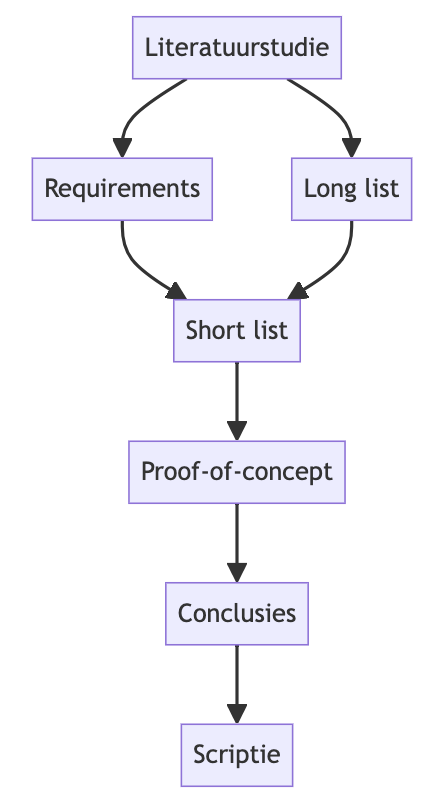
\includegraphics[scale=0.5]{methodologie.png}
\end{center}

%---------- Verwachte resultaten ----------------------------------------------
\section{Verwacht resultaat, conclusie}%
\label{sec:verwachte_resultaten}

Door te onderzoeken welke technologieën en oplossingen er al op de markt zijn in verband met master datakwaliteit kan er nagegaan worden of het al dan niet rendabel is om zelf een soortgelijke technologie op de markt te brengen. 

Het ontwikkelen van een nieuwe technologie en deze implementeren in SAP MDG Tool zal hoogstwaarschijnlijk wel rendabel zijn om zoiets op de markt te brengen. Dit is voornamelijk omdat veel bedrijven het nog steeds moeilijk hebben met het ordenen en managen van hun data. Dit is vaak doordat sommige data, zoals klantengegevens en productgegevens, door veel mensen gebruikt wordt en zo kunnen er verouderde gegevens of duplicaten ontstaan. Ook hebben nog niet veel IT-bedrijven een implementatie waarbij ML/AI de kwaliteit van artikel master data kan verhogen. Hierdoor is er nog niet veel concurrentie aanwezig op de markt, wat het ook weer veel aantrekkelijker maakt om zoiets zelf te implementeren. 

Door de proof-of-concept op te bouwen kan er veel makkelijker nagegaan worden of de data al dan niet al aanwezig is en deze desnoods moet aangepast worden. Hierdoor zouden de bedrijven veel minder duplicaten of verouderde gegevens bezitten in hun dataset en geen grote kosten meer moeten betalen om hun verwaarloosde dataset weer op punt te stellen. 



%%---------- Andere bijlagen --------------------------------------------------
% TODO: Voeg hier eventuele andere bijlagen toe. Bv. als je deze BP voor de
% tweede keer indient, een overzicht van de verbeteringen t.o.v. het origineel.
%\input{...}

%%---------- Backmatter, referentielijst ---------------------------------------

\backmatter{}

\setlength\bibitemsep{2pt} %% Add Some space between the bibliograpy entries
\printbibliography[heading=bibintoc]

\end{document}
